%==============================================================
%  lecons/algebre/ensemble_quotient.tex — Ensemble quotient
%==============================================================

\lecontitle{Ensemble quotient}{Algèbre — Relations d'équivalence et passage au quotient}

%=============================================================
%  § 1 — RELATIONS D'ÉQUIVALENCE
%=============================================================
\secnum{navyblue}{1}{Relations d'équivalence}

\begin{tcolorbox}[thmbox]
  \textbf{Définition.}\enspace%
  \index{relation d'équivalence}
  Une relation $\mathcal{R}$ sur un ensemble $E$ est une
  \emph{relation d'équivalence} si elle est :
  \begin{enumerate}
    \item \textbf{Réflexive :} $\forall x \in E,\; x\,\mathcal{R}\,x$ ;
    \item \textbf{Symétrique :} $\forall x,y \in E,\; x\,\mathcal{R}\,y \Rightarrow y\,\mathcal{R}\,x$ ;
    \item \textbf{Transitive :} $\forall x,y,z \in E,\; x\,\mathcal{R}\,y \text{ et } y\,\mathcal{R}\,z \Rightarrow x\,\mathcal{R}\,z$.
  \end{enumerate}
  La \emph{classe d'équivalence}\index{classe d'équivalence} de $x \in E$ est
  \[
    [x]_{\mathcal{R}} = \bigl\{y \in E \mid x\,\mathcal{R}\,y\bigr\}.
  \]
  Lorsque la relation $\mathcal{R}$ est sous-entendue, on note simplement $[x]$
  au lieu de $[x]_{\mathcal{R}}$.
\end{tcolorbox}

\rubriq{Classes et partition}

\begin{tcolorbox}[thmbox]
  \textbf{Théorème.}\enspace%
  \index{partition}
  \textit{Les classes d'équivalence de $\mathcal{R}$ forment une
  \emph{partition} de $E$ : elles sont deux à deux disjointes et leur
  réunion est $E$. Réciproquement, toute partition de $E$ définit
  une relation d'équivalence.}
\end{tcolorbox}

\begin{mdframed}[style=proofbar]
  \textit{Non-vide et recouvrement.} $x \in [x]$ par réflexivité, donc
  $E = \bigcup_{x\in E}[x]$.

  \textit{Disjonction.} Si $[x]\cap[y]\neq\emptyset$, soit $z\in[x]\cap[y]$.
  Alors $x\,\mathcal{R}\,z$ et $y\,\mathcal{R}\,z$, donc par symétrie et transitivité
  $x\,\mathcal{R}\,y$ (et, symétriquement, $y\,\mathcal{R}\,x$). Montrons les deux
  inclusions. Pour tout $t \in [x]$ : $x\,\mathcal{R}\,t$, et comme
  $y\,\mathcal{R}\,x$, la transitivité donne $y\,\mathcal{R}\,t$, soit $t\in[y]$ ;
  ainsi $[x]\subseteq[y]$. En échangeant les rôles de $x$ et $y$ dans le même
  raisonnement (on dispose aussi de $x\,\mathcal{R}\,y$), on obtient pour tout
  $t\in[y]$ que $t\in[x]$, soit $[y]\subseteq[x]$. Les deux inclusions donnent
  $[x]=[y]$. Ainsi deux classes sont \emph{égales ou disjointes}, donc deux à
  deux disjointes.

  \textit{Réciproque.} Étant donné une partition $(A_i)_{i\in I}$ de $E$, la
  relation « $x\,\mathcal{R}\,y$ si $x$ et $y$ appartiennent à un même $A_i$ »
  est réflexive, symétrique et transitive (chaque $x$ appartient à un unique
  bloc), et ses classes d'équivalence sont exactement les $A_i$. \hfill$\blacksquare$
\end{mdframed}

\decsep{}

%=============================================================
%  § 2 — ENSEMBLE QUOTIENT ET PROJECTION CANONIQUE
%=============================================================
\secnum{navyblue}{2}{Ensemble quotient et projection canonique}

\begin{tcolorbox}[thmbox]
  \textbf{Définition.}\enspace%
  \index{ensemble quotient}
  L'\emph{ensemble quotient} de $E$ par $\mathcal{R}$ est l'ensemble des
  classes d'équivalence :
  \[
    E/\mathcal{R} = \bigl\{[x] \mid x \in E\bigr\}.
  \]
  La \emph{projection canonique}\index{projection canonique} est l'application
  \[
    \pi : E \longrightarrow E/\mathcal{R}, \qquad x \longmapsto [x].
  \]
  Elle est surjective par définition.
\end{tcolorbox}

\begin{significationintuitive}
  Passer au quotient, c'est \emph{identifier} les éléments équivalents : on les
  « écrase » tous sur un même point. L'ensemble $E/\mathcal{R}$ est la vue de $E$
  où l'on ne distingue plus deux éléments reliés par $\mathcal{R}$, et la
  projection $\pi$ est l'application qui « oublie » cette distinction.
\end{significationintuitive}

\rubriq{Propriété universelle du passage au quotient}

\begin{tcolorbox}[thmbox]
  \textbf{Théorème (factorisation).}\enspace%
  \index{passage au quotient}
  \textit{Soit $f : E \to F$ une application. On dit que $f$ est
  \emph{compatible} avec $\mathcal{R}$ si}
  \[
    x\,\mathcal{R}\,y \;\Rightarrow\; f(x) = f(y).
  \]
  \textit{Dans ce cas, il existe une unique application
  $\bar{f} : E/\mathcal{R} \to F$ telle que $f = \bar{f} \circ \pi$,
  i.e.\ le diagramme}
  \[
    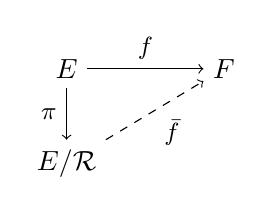
\begin{tikzpicture}[baseline=(current bounding box.center)]
      \node (E)  at (0,1)  {$E$};
      \node (F)  at (2,1)  {$F$};
      \node (Q)  at (0,-0.2) {$E/\mathcal{R}$};
      \draw[->] (E) -- node[above]{\small$f$} (F);
      \draw[->] (E) -- node[left]{\small$\pi$} (Q);
      \draw[->, dashed] (Q) -- node[below right]{\small$\bar{f}$} (F);
    \end{tikzpicture}
  \]
  \textit{est commutatif. De plus, $\bar{f}$ est injective si et seulement si
  $f(x)=f(y) \Rightarrow x\,\mathcal{R}\,y$.}
\end{tcolorbox}

\begin{mdframed}[style=proofbar]
  \textit{Existence et unicité.} On pose $\bar{f}([x]) = f(x)$.
  C'est bien défini : si $[x]=[y]$, alors $x\,\mathcal{R}\,y$, donc $f(x)=f(y)$.
  L'unicité vient de $f = \bar{f}\circ\pi$ : on doit avoir $\bar{f}([x]) = f(x)$.

  \textit{Injectivité ($\Leftarrow$).} Supposons que $f(x)=f(y)\Rightarrow x\,\mathcal{R}\,y$.
  Alors $\bar{f}([x])=\bar{f}([y]) \Rightarrow f(x)=f(y)
  \Rightarrow x\,\mathcal{R}\,y \Rightarrow [x]=[y]$, donc $\bar{f}$ est injective.

  \textit{Injectivité ($\Rightarrow$).} Réciproquement, si $\bar{f}$ est injective
  et $f(x)=f(y)$, alors $\bar{f}([x])=\bar{f}([y])$ (puisque $\bar{f}([z])=f(z)$),
  d'où $[x]=[y]$ par injectivité, c'est-à-dire $x\,\mathcal{R}\,y$. \hfill$\blacksquare$
\end{mdframed}

\decsep{}

%=============================================================
%  § 3 — EXEMPLES FONDAMENTAUX
%=============================================================
\secnum{navyblue}{3}{Exemples fondamentaux}

\begin{mdframed}[style=exbar]
  \textbf{1. Congruences : $\mathbb{Z}/n\mathbb{Z}$.}\enspace%
  \index{congruence}\index{$\mathbb{Z}/n\mathbb{Z}$}
  Sur $\mathbb{Z}$, poser $a \equiv b \pmod{n}$ si $n \mid (b-a)$.
  C'est une relation d'équivalence ; la classe de $a$ est
  $[a] = \{a + kn \mid k \in \mathbb{Z}\}$.
  L'ensemble quotient $\mathbb{Z}/n\mathbb{Z} = \{[0],[1],\ldots,[n-1]\}$
  est un anneau (et même un corps si $n$ est premier).

  \smallskip\noindent
  \textbf{2. Construction de $\mathbb{Q}$.}\enspace%
  \index{nombres rationnels!construction}
  Sur $\mathbb{Z}\times\mathbb{Z}^*$, poser $(a,b)\sim(c,d)$ si $ad = bc$.
  C'est une relation d'équivalence, et
  $\mathbb{Q} = (\mathbb{Z}\times\mathbb{Z}^*)/{\sim}$.
  La classe de $(a,b)$ est notée $\tfrac{a}{b}$.

  \smallskip\noindent
  \textbf{3. Espace vectoriel quotient.}\enspace%
  \index{espace vectoriel quotient}
  Soit $F$ un sous-espace de $E$. On pose $x \sim y$ si $x-y \in F$.
  L'ensemble quotient $E/F$ est naturellement un $\mathbb{K}$-espace vectoriel,
  et lorsque $E$ est de dimension finie, $\dim(E/F) = \dim E - \dim F$
  (propriété du quotient).

  \smallskip\noindent
  \textbf{4. Orbites d'une action de groupe.}\enspace%
  \index{orbite}
  Si un groupe $G$ agit sur $E$, poser $x \sim y$ si $\exists\,g \in G,\, y=g\cdot x$.
  Les classes sont les \emph{orbites} ; $E/{\sim}$ est l'espace des orbites.
\end{mdframed}

\decsep{}

%=============================================================
%  § 4 — APPLICATIONS, PIÈGES, EXERCICES
%=============================================================
\secnum{exgreen}{4}{Applications, pièges et exercices}

\rubriq{Pièges}

\begin{mdframed}[style=cexbar]
  \textbf{Bien-fondé des opérations.}\enspace%
  Pour définir une loi sur $E/\mathcal{R}$, il faut vérifier que l'opération
  ne dépend pas du représentant choisi.
  Exemple piège : sur $\mathbb{Z}$, la relation $a\sim b$ si $|a|=|b|$ est
  une relation d'équivalence, mais $[a]+[b]:=[a+b]$ n'est \emph{pas} bien définie.
  En effet $1\sim{-1}$, donc $[1]=[{-1}]$. Calculons $[1]+[1]$ :
  avec le représentant $1$, on obtient $[1+1]=[2]$ ;
  avec le représentant $-1$, on obtient $[{-1}+1]=[0]$.
  Or $[2]=\{2,-2\}\neq\{0\}=[0]$ : le résultat dépend du choix du représentant.

  \smallskip\noindent
  \textbf{$E/\mathcal{R}$ peut être très grand ou très petit.}\enspace%
  Si $\mathcal{R}$ est l'égalité, $E/\mathcal{R} \cong E$.
  Si $\mathcal{R}$ est la relation grossière ($x\,\mathcal{R}\,y$ toujours), $E/\mathcal{R}$
  est un singleton.
\end{mdframed}

\vspace{6pt}
\exolabel

\begin{mdframed}[style=exobar]
  \begin{enumerate}
    \item Montrer que la relation $\sim$ sur $\mathbb{R}^2$ définie par
          $(x,y)\sim(x',y')$ si $x^2+y^2=x'^2+y'^2$ est une relation
          d'équivalence. Décrire $\mathbb{R}^2/{\sim}$ et la projection canonique.

    \item Soit $f : E \to F$. Montrer que la relation $x\sim_f y \Leftrightarrow f(x)=f(y)$
          est une relation d'équivalence, et que l'application induite
          $\bar{f} : E/{\sim_f} \to F$ est injective. En déduire la décomposition
          canonique $f = \iota \circ \bar{f} \circ \pi$ où $\iota$ est l'injection
          de $\mathrm{Im}(f)$ dans $F$.

    \item Montrer que $\mathbb{Z}/n\mathbb{Z}$ est un corps si et seulement si
          $n$ est premier.

    \item Soit $E = \mathcal{C}([0,1],\mathbb{R})$ et $f \sim g$ si $\int_0^1 f = \int_0^1 g$.
          Montrer que c'est une relation d'équivalence. Décrire $E/{\sim}$.

    \item (Théorème de Noether) Soit $\varphi : G \to H$ un homomorphisme de groupes.
          Montrer que $G/\ker\varphi \cong \mathrm{Im}(\varphi)$.
  \end{enumerate}
\end{mdframed}

\leconfooter{G.\ Cantor (1874) — B.\ Russell (1903) — structures quotient omniprésentes en algèbre}
